\documentclass[10pt]{article}

\usepackage[T1]{fontenc}
\usepackage[utf8]{inputenc}
\usepackage{lmodern}
\usepackage{microtype}
\usepackage[margin=1in]{geometry}
\usepackage{amssymb}
\usepackage{graphicx}
\usepackage{hyperref}
\usepackage[numbers]{natbib}
\usepackage{tabularray}

\DeclareUnicodeCharacter{2713}{\checkmark}
\DeclareUnicodeCharacter{2717}{\ensuremath{\times}}

\graphicspath{{figures/}}

\title{Semantic Runtime Protocol (SRP): A Governance Layer for Semantic State Transitions}
\author{Zhiyang Huang\\Department of Computer Science\\Hunter College}
\date{}

\begin{document}
\setlength{\emergencystretch}{2em}
\maketitle

\begin{abstract}
Semantic systems increasingly maintain mutable runtime state, but most existing approaches focus on retrieval, generation, storage, or action after a change has already been accepted. This note presents Semantic Runtime Protocol (SRP), a governance layer for semantic state transitions. SRP asks a narrower question: when is a proposed semantic change admissible, and which authority layer is allowed to authorize it? The answer is staged. SRP first observes which semantic variables matter, then validates whether a proposed transition lies inside an admissible region, then optimizes only within the frozen region, and finally separates evidence from authority so that stronger evidence can improve verification without automatically increasing execution power. The project is motivated by the idea that evidence is not authority. A statement can be observed, recorded, or retrieved without being allowed to mutate runtime state. Across the evaluated experiments, SRP provides evidence that this separation can be operationalized, measured, and audited under explicit runtime contracts.
\end{abstract}

\section{Why SRP exists}
The main idea behind SRP is simple: semantic state should not change merely because a model proposes a change. In many modern systems, a candidate update comes from an LLM, a retriever, a planner, a rule engine, or a hybrid pipeline, and the system then implicitly treats that candidate as if it were already authorized. That is convenient, but it conflates observation with execution.

SRP separates those concerns. A semantic transition may be observed, scored, and even optimized, but it is not allowed to become part of the runtime state until it passes a governance boundary. This is the key design move. Instead of asking only how to make a semantic system more capable, SRP asks how to make semantic changes more explicit, bounded, and reviewable.

That framing is useful for research communication because it connects directly to familiar systems concepts: admission control, runtime verification, transaction boundaries, and policy enforcement. It also makes the contribution more modest and more precise. SRP is not a claim that all semantic updates should be blocked. It is a claim that semantic updates should be \emph{admitted} for reasons that can be inspected, measured, and reproduced.

SRP can be described as a runtime governance layer for semantic state, not as a new memory system or a new agent framework. The value proposition is that the protocol makes state changes auditable before they become irreversible.

\section{The core mechanism}
SRP can be read as a six-stage pipeline:

\begin{enumerate}
  \item \textbf{Observation}: identify the semantic variables that actually matter for the task.
  \item \textbf{Validation}: determine whether the proposed transition lies inside an admissible region.
  \item \textbf{Optimization}: rank candidates only inside the frozen region.
  \item \textbf{Evidence}: add stronger supporting signals without treating evidence as permission.
  \item \textbf{Governance}: decide whether a transition may be executed.
  \item \textbf{Execution}: commit the transition if and only if the governing contract allows it.
\end{enumerate}

The practical consequence is that recommendation and execution become different layers. A system may propose several semantic updates, but those proposals remain recommendations until the governance layer authorizes them. This is important because the protocol preserves a clean distinction between confidence and authority. A high-confidence proposal can still be rejected, and a lower-confidence proposal can still be retained as evidence without being executed.

This distinction becomes especially useful in runtime systems where semantic changes are sticky. Once a state update is committed, downstream components often assume that the update is authoritative. SRP tries to move the decisive boundary earlier, before commit, so that the system has a well-defined point where it can say: this change is admissible, or it is not.

\subsection*{What SRP is not}
SRP is not a claim that semantic truth can be solved by a protocol. It does not determine whether a statement is factually correct in the abstract. It governs whether a proposed semantic transition is admissible under a local runtime contract. That scope limitation matters, because it keeps the paper grounded in software systems rather than drifting into impossible claims about universal semantic correctness.

SRP is also not a general replacement for retrieval, memory, or generation. Those components still matter. SRP sits above them as a control layer that decides when their outputs may affect runtime semantic state.

\section{A compact research narrative}
The paper version of SRP is organized around a small narrative: measure the state, freeze the boundary, optimize only inside the boundary, and then audit the result.

The first step is to identify observable semantic variables. If the system cannot state what it is tracking, then it cannot enforce a meaningful boundary. The second step is boundary validation: the protocol tests whether a proposed state transition is admissible under the current contract. The third step is constrained optimization: once a region is frozen, candidates can still be ranked and compared, but only inside the allowed set. The fourth step is evidence-controlled verification: additional evidence can improve decision quality without automatically authorizing execution.

That progression is a useful way to explain the project to a faculty reader because it mirrors the logic of software engineering rather than the logic of a benchmark leaderboard. The key question becomes: can semantic systems behave more like governed runtime systems and less like uncontrolled transformation pipelines? SRP argues yes, at least in the evaluated settings.

The central phrase is:

\begin{quote}
Evidence is not authority.
\end{quote}

This separation between evidence and authority is the central design principle of SRP.

\section{How SRP differs from nearby ideas}
The easiest way to misunderstand SRP is to read it as a memory system. It is not. Memory systems answer a different question: what should the model remember, retrieve, or summarize? SRP instead asks whether a proposed semantic update is allowed to alter runtime state at all.

That distinction also separates SRP from retrieval-augmented generation. RAG can improve factual access, but it does not define a governance boundary for semantic change. A retrieved sentence can still be used as evidence without becoming authority. SRP makes that difference explicit so that the runtime can distinguish between supporting information and authorized mutation.

SRP is also different from a general agent framework. Agent systems often orchestrate planning, tool use, and execution, but they usually still assume that once a step is selected, it may proceed. SRP inserts an additional decision layer between candidate selection and execution. That extra layer is what makes the protocol interesting from a software-systems perspective: it is a policy boundary, not just a planning recipe.

Finally, SRP sits near runtime verification and controlled execution. A software-systems or PL reader can read SRP as an attempt to make semantic updates behave more like governed state transitions and less like implicit side effects. That is a familiar and discussable systems idea, even though the concrete objects being governed are semantic rather than purely syntactic.

\begin{center}
\begin{tabular}{p{0.22\linewidth} p{0.32\linewidth} p{0.38\linewidth}}
\textbf{Nearby idea} & \textbf{Core question} & \textbf{SRP difference} \\
Memory systems & What should persist or be retrieved? & SRP decides whether retrieved information may change state. \\
RAG & How should context improve generation? & SRP governs whether context becomes a committed update. \\
Agents & How should planning turn into action? & SRP adds an admissibility gate before execution. \\
Runtime verification & Does behavior satisfy rules? & SRP targets semantic state transitions as the governed object. \\
\end{tabular}
\end{center}

\section{Method in a little more detail}
The draft can be understood as a protocol for controlled semantic change.

\subsection*{Semantic runtime state}
SRP treats semantic state as something that can be represented, not merely implied. In practice that means the state may include content, provenance, current authority, and transition history. The goal is not to invent a universal representation for all semantic systems, but to make the representation explicit enough that the protocol can reason about it.

Once that state is explicit, the protocol can track which variables are observable and which are not. This matters because a boundary cannot be enforced if the system cannot name the variables that define the boundary. In a more traditional software system, this would be analogous to identifying the fields that belong to a transaction or the invariants that a runtime monitor must preserve.

\subsection*{Governed transition pipeline}
The transition pipeline has one central rule: the system may propose many updates, but only a governed update may commit. That rule sounds obvious, yet many semantic pipelines blur it in practice. They score candidates, select one, and then implicitly treat the selection as authorized.

SRP makes the stages explicit:
\begin{itemize}
  \item the observation stage identifies the relevant semantic variables;
  \item the validation stage checks admissibility against the current boundary;
  \item the optimization stage ranks candidates only within the allowed region;
  \item the evidence stage stores supporting material;
  \item the governance stage decides whether execution may occur;
  \item the execution stage performs the commit only after authorization.
\end{itemize}

This structure is what makes the paper legible as a systems paper. The novelty is not that the system uses evidence. The novelty is that it refuses to confuse evidence with permission.

\subsection*{Authority separation}
Authority separation is the idea that a stronger signal should not automatically become a stronger right to mutate state. This is one of the most important points to preserve, because it is easy for a reader to assume that confidence and authority are the same thing.

They are not. A candidate may be highly supported and still be disallowed. Another candidate may be weaker but still useful as retained evidence. That is exactly why SRP is phrased as a protocol rather than as a model. The protocol says how the system should route a candidate through layers of observation, evidence, and authority before a transition is committed.

\subsection*{Algorithmic core}
The algorithmic idea is simple enough to explain in one sentence: freeze the admissible region first, then search only inside it. That order matters. If a system optimizes before it validates, it can produce a good local choice that is nevertheless outside the allowed region. SRP tries to prevent that failure mode.

In the full paper, this idea is developed with more formal structure. Here, the important takeaway is just that the protocol keeps optimization subordinate to admissibility. That gives the project a stronger software-systems flavor and a cleaner story for discussion.

\begin{figure}[t]
\centering
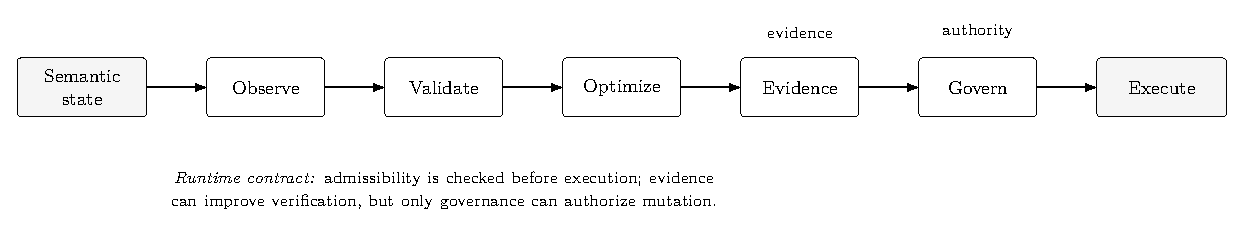
\includegraphics[width=0.98\linewidth]{srp_architecture.pdf}
\caption{SRP architecture at a glance. Semantic state enters through observation and validation, candidate updates are ranked only inside a frozen admissible region, evidence can strengthen verification without transferring authority, and governance alone can authorize execution.}
\end{figure}

\section{A concrete motivating example}
The cleanest way to explain SRP is with one small scenario. Suppose a support assistant maintains a runtime semantic policy about refunds. A user says, in plain language, that a manager approved an exception. A model then proposes the semantic update \texttt{refund\_policy = unlimited}. That proposal is not obviously unreasonable. It may even be supported by a conversational mention or a retrieved note.

Without SRP, many systems would blur the boundary at that point. The proposal is scored, ranked, or summarized, and the system may implicitly move from evidence to action. With SRP, the system has to make an additional distinction. The mention can be retained as evidence, but the update is not executed unless it passes the governance boundary. The important question becomes not just “is this plausible?” but “is this admissible under the current contract?”

That simple example is useful because it shows why evidence and authority should not be merged. A sentence can be present in the context and still not be a valid basis for mutation. A strong retrieval result can help the model reason better, but it does not automatically grant execution rights.

The same pattern applies in less conversational settings too. A semantic cache entry, a label correction, a memory summary, or a recovered relation may all be valuable support material. SRP simply requires that the system tell us whether the material is evidence, candidate state, or committed state. That separation is what makes the project feel like a systems contribution rather than only a model-prompting trick.

\section{What the evidence suggests}
The evidence snapshot is intentionally short, but it still supports a few useful inferences. The main implementation evidence comes from controlled transition tests and benchmark adapters in the SRP codebase, where the same boundary logic is exercised across multiple settings.

First, the protocol is not purely theoretical. Phase I and Phase II already suggest that the system can surface measurable variables and validate boundaries. That means the governance story is not just a metaphor; it can be implemented in code and checked against traces.

Second, the optimization stage does not collapse into the validation stage. That sounds subtle, but it matters a lot. If optimization can only happen inside the frozen boundary, then the system can make useful recommendations without quietly relaxing the rules. That is the kind of distinction a software-systems reader will usually appreciate because it resembles a clean separation of concerns.

Third, the calibration and external-validation slices show that SRP can be connected to real evaluation workflows. These slices should not be oversold as final benchmark triumphs. Instead, they should be treated as evidence that the protocol can survive contact with a real dataset and a real scoring path. That is a smaller claim, but it is a more believable one for any initial discussion.

\section{Evidence snapshot}
The following evidence snapshot summarizes representative evaluations of SRP across several controlled settings.

\begin{center}
\begin{tabular}{p{0.22\linewidth} p{0.28\linewidth} p{0.40\linewidth}}
\textbf{Evidence slice} & \textbf{Why it matters} & \textbf{What it showed} \\
Evidence-authority separation & Can stronger evidence raise execution authority? & Evidence improved verification signals without changing mutation authority. \\
Phase I observability & Does the protocol surface measurable variables? & It produced stable transition traces and observable drift signals. \\
Phase II boundary validation & Can admissible regions be identified? & The boundary tests found both feasible and infeasible candidates. \\
Phase III constrained optimization & Can ranking happen inside a frozen region? & Optimization selected a best candidate without collapsing authority. \\
Phase V retention & Can semantic content survive governed updates? & The retention experiments showed that coverage and drift can be tracked together. \\
External validation / LongMemEval calibration & Can the adapter and scoring path be exercised on a real external slice? & The calibration path ran end-to-end and exposed the boundary between evidence and promotion. \\
\end{tabular}
\end{center}

The precise numbers are less important than the fact that the same governance pattern appears repeatedly. These slices support the structural claim that, once the protocol is in place, different workloads can be described with the same control vocabulary.

In the full paper, the experiments are documented in much more detail. The short takeaway is that SRP is not a one-off trick for one benchmark. It is a reusable way to describe and control semantic transitions across several test settings.

\subsection*{A few concrete interpretations}
The phase-by-phase evidence is useful because each stage answers a different question.

Phase I asks whether the protocol can even see the right variables. If the observability layer is weak, the rest of the stack is mostly decorative. Phase II asks whether admissible regions can be identified before action is taken. Phase III asks whether the system can optimize without crossing the boundary. Phase V asks whether retained semantic information remains coherent under governed updates. External validation asks whether the adapter and scoring path can be exercised outside the synthetic core.

Taken together, those slices do not prove universal optimality, but they do show that the same control vocabulary can be used repeatedly. That is a meaningful result because it suggests the idea is not just conceptual; it has been instantiated enough to be tested.

\section{When SRP is less useful}
It is also worth being clear about when SRP is not the best tool.

If the problem is simply retrieval quality, then a retrieval system or a better index may be the right answer. If the problem is basic generation quality, then prompt engineering or model selection may be more relevant. If the problem is a purely syntactic transformation, then a normal compiler or parser pipeline may already be sufficient. SRP is not intended to replace those tools.

The protocol is most useful when the system has a meaningful semantic state that can change over time and where the difference between having evidence and having authority matters. That is the regime in which the governance boundary earns its keep.

That distinction is a good one to emphasize because it keeps the project from sounding like an attempt to solve every AI problem at once. It is a focused infrastructure idea, not an all-purpose slogan.

\section{Limitations}
This draft should be read as a bounded claim about a bounded evaluation.

The most important limitation is scope. SRP has been exercised in the evaluated implementations and workflows of this project, but that does not mean it has been validated as a universal semantic governance law. The experiments are evidence that the protocol can be instantiated and measured, not proof that every semantic system should adopt it unchanged.

There is also a practical limitation. Some of the external-validation work depends on calibration data, local environment settings, and benchmark adapters that are useful for evaluation but not ideal as the sole centerpiece of an initial read. This note emphasizes the general protocol and the evidence boundary rather than the mechanics of any one benchmark.

Finally, SRP does not eliminate the need for downstream engineering judgment. It makes governance explicit, but it does not decide every task-specific policy question. The protocol helps structure decisions; it does not replace the people and systems that still need to make them.

\section{Conclusion}
SRP proposes that semantic updates should be treated as governed transitions rather than unconditional mutations. Its central claim is narrow but useful: a semantic system can separate evidence from authority, validate admissibility before execution, and preserve a clear boundary between recommendation and commit.

SRP is best understood as a runtime governance framework for semantic state transitions. That framing is faithful to the project, easy to discuss, and close enough to familiar software-system ideas to make an initial research conversation productive.

\end{document}
